\part{Algorithms} \label{part:three algorithms}

\chapter{T-distributed Stochastic Neighbor Embedding (T-SNE)}

\section{Background}

some related work and background

\section{Asymmetric SNE}

Given N observations of some high dimensional data, for any pair, $x_i$ and $x_j$, SNE defines the similarity (aka an affinity or weight) between them, using a Gaussian kernel function:

\begin{equation*}
    {v_{i\mid j}} = \exp {(-\beta_i r^2_{ij})} 
\end{equation*}

\noindent Where $r_i_j$ is the distance between $x_i$ and $x_j$ and $\beta_i$ must be determined by some method. The notation of $v_{i \mid j}$ rather than $v_i_j$, is to indicate that this quantity is not symmetric, i.e. $v_{i \mid j} \neq v_{j \mid i}$. This notation is from the conditional versus joint probability definitions used in symmetric SNE (see below). The $r_i_j$ notation indicates that the distances are symmetric.\\

\noindent The weights are normalized to form $N$ probability distributions:

\begin{equation*}
    {p_{j\mid i}} = \frac {v_{j\mid i}} {\sum_k^N v_{k\mid i}}
\end{equation*}

\noindent $\beta_i$ is chosen by finding that value that results in the probability distribution having a specific perplexity. The perplexity has to be chosen by the user, but is interpreted as being a continuous version of the number of nearest neighbors, and generally is chosen to take values between 5 and 50. $p_{j\mid i}$ is a conditional probability, and is interpreted as the probability that item j will be chosen as being similar to item i, given that item i was picked already.

\noindent At the same time, the output space of the embedded coordinates, which is the similarity between the points $y_i$ and $y_j$ is also defined as a Gaussian:

\begin{equation*}
    {{w_i_j} = \exp {(-d^2_{ij})} }
\end{equation*}

\noindent $d_i_j$ is the Euclidean distance between $y_i$ and $y_j$. There is no $\beta$ in this weight definition so these weights are symmetric. The output probabilities, $q_{j\mid i}$ are calculated from $w_i_j$ in the same way that we go from ${v_{j\mid i}}$ to ${p_{j\mid i}}$, again creating N probability distributions. Due to normalizing by rows, the $q_{j\mid i}$ are asymmetric despite the symmetric weights they are generated from.\\

\noindent Therefore, The SNE cost function could be defined as the sum of the Kullback-Leibler divergences of the N distributions:

\begin{equation*}
    {C_S_N_E} = {\sum_i KL(P_i \mid \mid Q_i)} =  { {\sum_i^N} {\sum_j^N} {p_{j\mid i}} \log \frac{p_{j\mid i}}{q_{j\mid i}} }
\end{equation*}

Because KL distance is an asymmetric scale. The purpose of minimizing the cost function is to make the values of $p_{j∣i}$ and $q_{j∣i}$ as close as possible,  that is, the similarity of points in the low-dimensional space is consistent with the similarity of points in the high-dimensional space. But it can be trimmed from the form of the cost function. When $p_{j∣i}$ is relatively bigger and $q_{j∣i}$  is relatively smaller, the cost is higher; when $p_{j∣i}$ is smaller and $q_{j∣i}$ is bigger, the cost is lower. This means when two data points in a high-dimensional space are relatively close, if they are mapped to a low-dimensional space and are farther apart, then they will get a high penalty, which is of course no problem. Conversely, when the two data points in the high-dimensional space are farther apart, if they are mapped to the low-dimensional space, they will get a very low penalty value. This is a problem, and it should be a higher penalty. In other words, the cost function of SNE pays more attention to the local structure rather than global impact.

\section{Symmetric SNE}
In Symmetric SNE, the input probability matrix is symmetrized by averaging pj|i and pi|j and then re-normalized over all pairs of points, to create a single (joint) probability distribution, $p_i_j$:

\begin{equation*}
    {p_{i j}} = \frac {p_{i\mid j} + p_{j\mid i}} {2N}
\end{equation*}

\noindent The output probabilities, $q_i_j$ are now defined by normalizing the output weights over all pairs, again creating a single probability distribution:

\begin{equation*}
    {q_{i j}} = \frac {w_{i j}} {\sum_k^N \sum_l^N w_{k l}}
\end{equation*}

\noindent Where $N$ is the total number of data points, this definition not only satisfies the symmetry, but also ensures that the penalty value of xi will not be too small. Which maens no matter where the outlier's mapping point in low dimension $y_i$ in the space is at any position, the penalty value can be guaranteed. At this time, the following cost function can be written using KL distance:

\begin{equation*}
    {C_S_S_N_E} = {\sum_i KL(P \mid \mid Q)} =  { {\sum_i^N} {\sum_j^N} {p_{i j}} \log \frac{p_{i j}}{q_{i j}} }
\end{equation*}

\noindent In the end, the result for UPS database, which has five kind of image of hand writing can be seen as below:

\begin{figure}[ht]

\centering
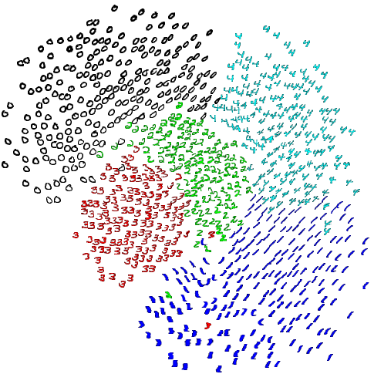
\includegraphics[scale=1.5]{images/image_SNE.png}
\caption{result of SNE algorithm for UPS dataset}
\label{fig:label}
\end{figure}

\section{The Crowding Problem}

As we can observe from the image above, the dimension reduction result is satisfied, which means different kinds of images can be clustered by each category. However, the boundary between each cluster is not clear enough. It would be hard to tell the difference if there is no marks in different color for each group, which is also not convenient for data visualization.\\  

\noindent Part of the reason of this situation is the SNE algorithm pays more attention to the local structure than the global structure. The more important reason could be the difference between the high-dimensional space distance distribution and the low-dimensional space distance distribution. With the increase of the dimensions, the sparseness of high-dimensional spatial data will also increase because the volume increases exponentially.\\

\noindent If there is An $m$-dimensional sphere with radius $r$ centered on data point $x_i$, its space increase with $r^m$. Assuming that the data points are uniformly distributed in the m-dimensional sphere, The distance between other data points and $x_i$ as the dimension increases could be observed as below:

\begin{figure}[ht]

\centering
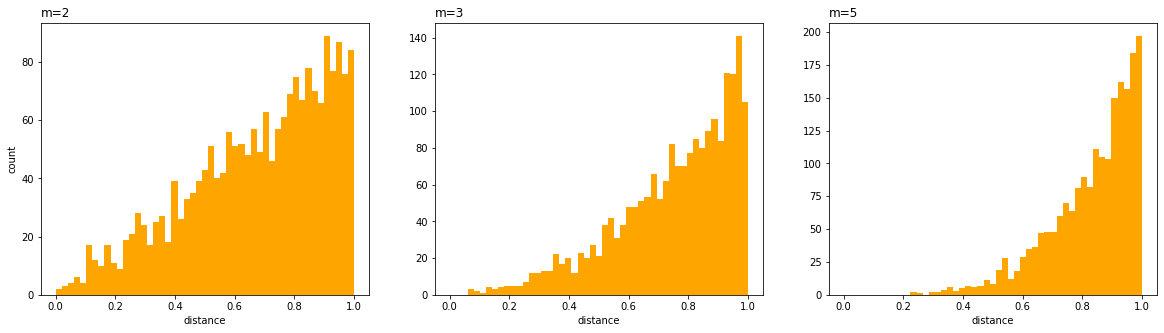
\includegraphics[scale=0.34]{images/image_crowding_problem_1.png}
\caption{distribution of distances between $x_i$ with dimension 2 to 5}
\label{fig:label}
\end{figure}

\begin{figure}[ht]

\centering
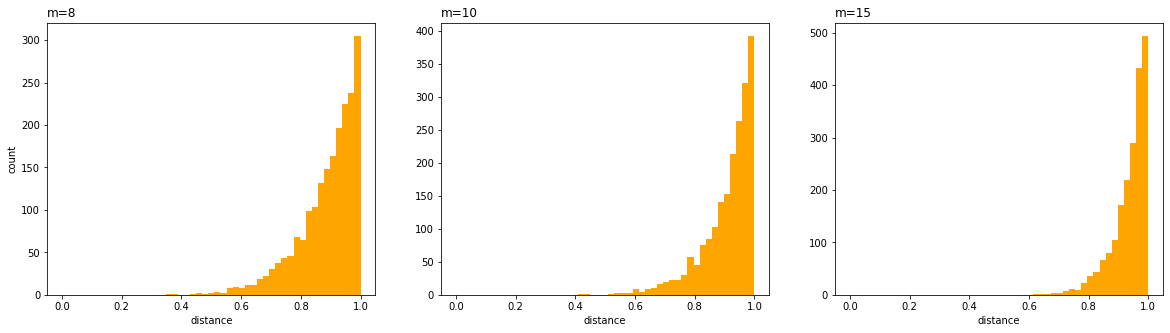
\includegraphics[scale=0.34]{images/image_crowding_problem_2.png}
\caption{distribution of distances between $x_i$ with dimension 8 to 15}
\label{fig:label}
\end{figure}

\noindent It can be observed from the figure that as the dimension increases, most of the data points are clustered near the surface of the sphere, and the distance distribution from the point $x_i$ is extremely uneven. If this distance relationship is directly retained to a low dimension, there will be a crowding problem.

\section{T-SNE}
Draw a random sample with a capacity of $N$ from the normal population. If the mean of the normal population is $μ$, the variance is $\sigma^2$. The mean of the random sample is $\bar{x}$, and the variance is $s^2=  \frac {1}{N−1} \sum ^N_{i=1} (x_i−\bar{x})^2$, and the random variable t can be expressed as:

\begin{equation*}
    {t} =  \frac {\bar{x} - \mu}{s / \sqrt{N}} 
\end{equation*}

\noindent $t$ satisfies the t distribution with n−1 degrees of freedom, written as, $t∼t(n−1)$. t distribution is a typical long-tailed distribution. It is relatively gentle at both ends of the tail, which has obvious advantages when dealing with small samples and abnormal points.

\begin{figure}[ht]

\centering
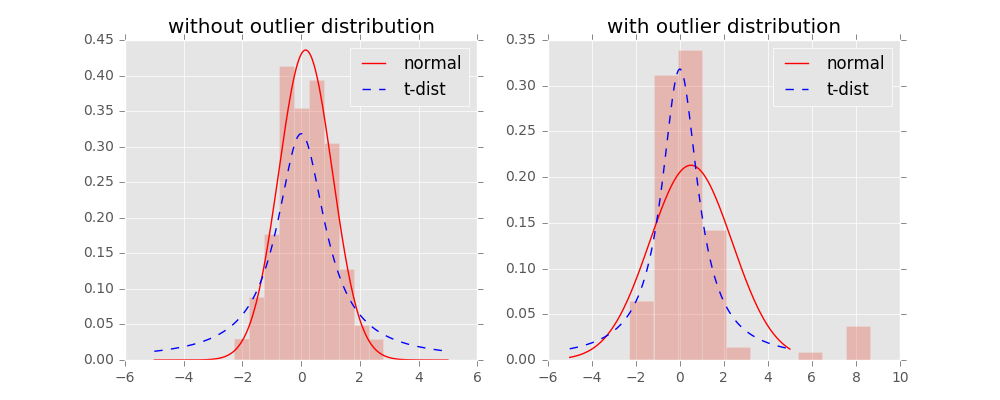
\includegraphics[scale=0.6]{images/image_t-distribution.png}
\caption{normal distribution and t distribution with and with out outliers}
\label{fig:label}
\end{figure}

\noindent From the graph 2.4, it can be easily observed that when there are no outliers, the fitting result of t distribution and Gaussian distribution are basically consistent. In the second picture, there are some abnormal points. Because the tail of the Gaussian distribution is low, it is more sensitive to abnormal points. In order to take care of these abnormal points, the fitting result of the Gaussian distribution deviates from the location of most samples, and the variance is also large. In contrast, the tail of the t distribution is relatively high and it is not sensitive to outliers, that ensure its robustness, so its fitting results are more reasonable, and the overall characteristics of the data are better captured.

\noindent With the t distribution now, for points that are close in high-dimensional space, in order to satisfy $p_i_j$=$q_i_j$, the distance in low-dimensional space needs to be slightly smaller; and for points that are far apart in high-dimensional space, in order to satisfy $p_i_j$=$q_i_j$, in low-dimensional space The distance needs to be farther. Then, We redefine the weight function from symmetric SNE: 

\begin{equation*}
    {w_i_j} =  \frac {1}{1+d_i_j^2} 
\end{equation*}

\noindent Barnes-Hut t-SNE has optimized the speed of traditional t-SNE, and it has some differences from traditional t-SNE:\\

\noindent 1. the gradient calculation algorithm uses Barnes-Hut approximation running in O(NlogN) time while the original T-SNE algorithm in O($N^2$) time. The exact algorithm should be used when nearest-neighbor errors need to be better than 3$\%$

\noindent 2.Barnes-Hut only works when the target dimension is 3 or less. Focus on 2D visualization.

\noindent 3. Barnes-Hut is an approximation. Use the angle parameter to control the approximation\\

\noindent Since the result from these two algorithm have similar accuracy and Barnes-Hut T-SNE is much faster than another. This thesis will focus the performance and characteristics of it.

\chapter{LargeVis}
\section{KNN tree}

LargeVis takes a different approach: it re-uses a lot of the same definitions as t-SNE, but makes sufficient modifications so that it’s possible to use stochastic gradient descent.\\

disadvantages of T-SNE\\
\\
modifications from T-SNE\\

\chapter{Umap}


testtesttest\\

\chapter{Assessment Algorithm}


testtesttest\\